\documentclass[14pt]{beamer}
%\usepackage{czech}
\usepackage[utf8]{inputenc}

\usepackage{utopia} %font utopia imported



\usetheme{Madrid}
\usecolortheme{default}

\usepackage{pgfpages}

\setbeameroption{hide notes}
%\setbeameroption{show only notes} % Only notes
%\setbeameroption{show notes on second screen=right} % Both

%------------------------------------------------------------
%This block of code defines the information to appear in the
%Title page
\title[Školení Laser] %optional
{Školení Laser}

\subtitle{Industra LABS Training Series}

\author[Šimon Berka] % (optional)
{Šimon Berka\inst{1} \and Industra LABS\inst{2}}



\date[2019] % (optional)
{2019}



%End of title page configuration block
%------------------------------------------------------------



%------------------------------------------------------------
%The next block of commands puts the table of contents at the 
%beginning of each section and highlights the current section:

\AtBeginSection[]
{
	\begin{frame}
	\frametitle{Obsah školení}
	\tableofcontents[currentsection]
\end{frame}
}
%------------------------------------------------------------


\begin{document}

%The next statement creates the title page.
\frame{\titlepage}


%---------------------------------------------------------
%This block of code is for the table of contents after
%the title page
\begin{frame}
\frametitle{Obsah školení}
\tableofcontents
\end{frame}
%---------------------------------------------------------

\begin{frame}
\frametitle{Individuální test laseru}
\centering
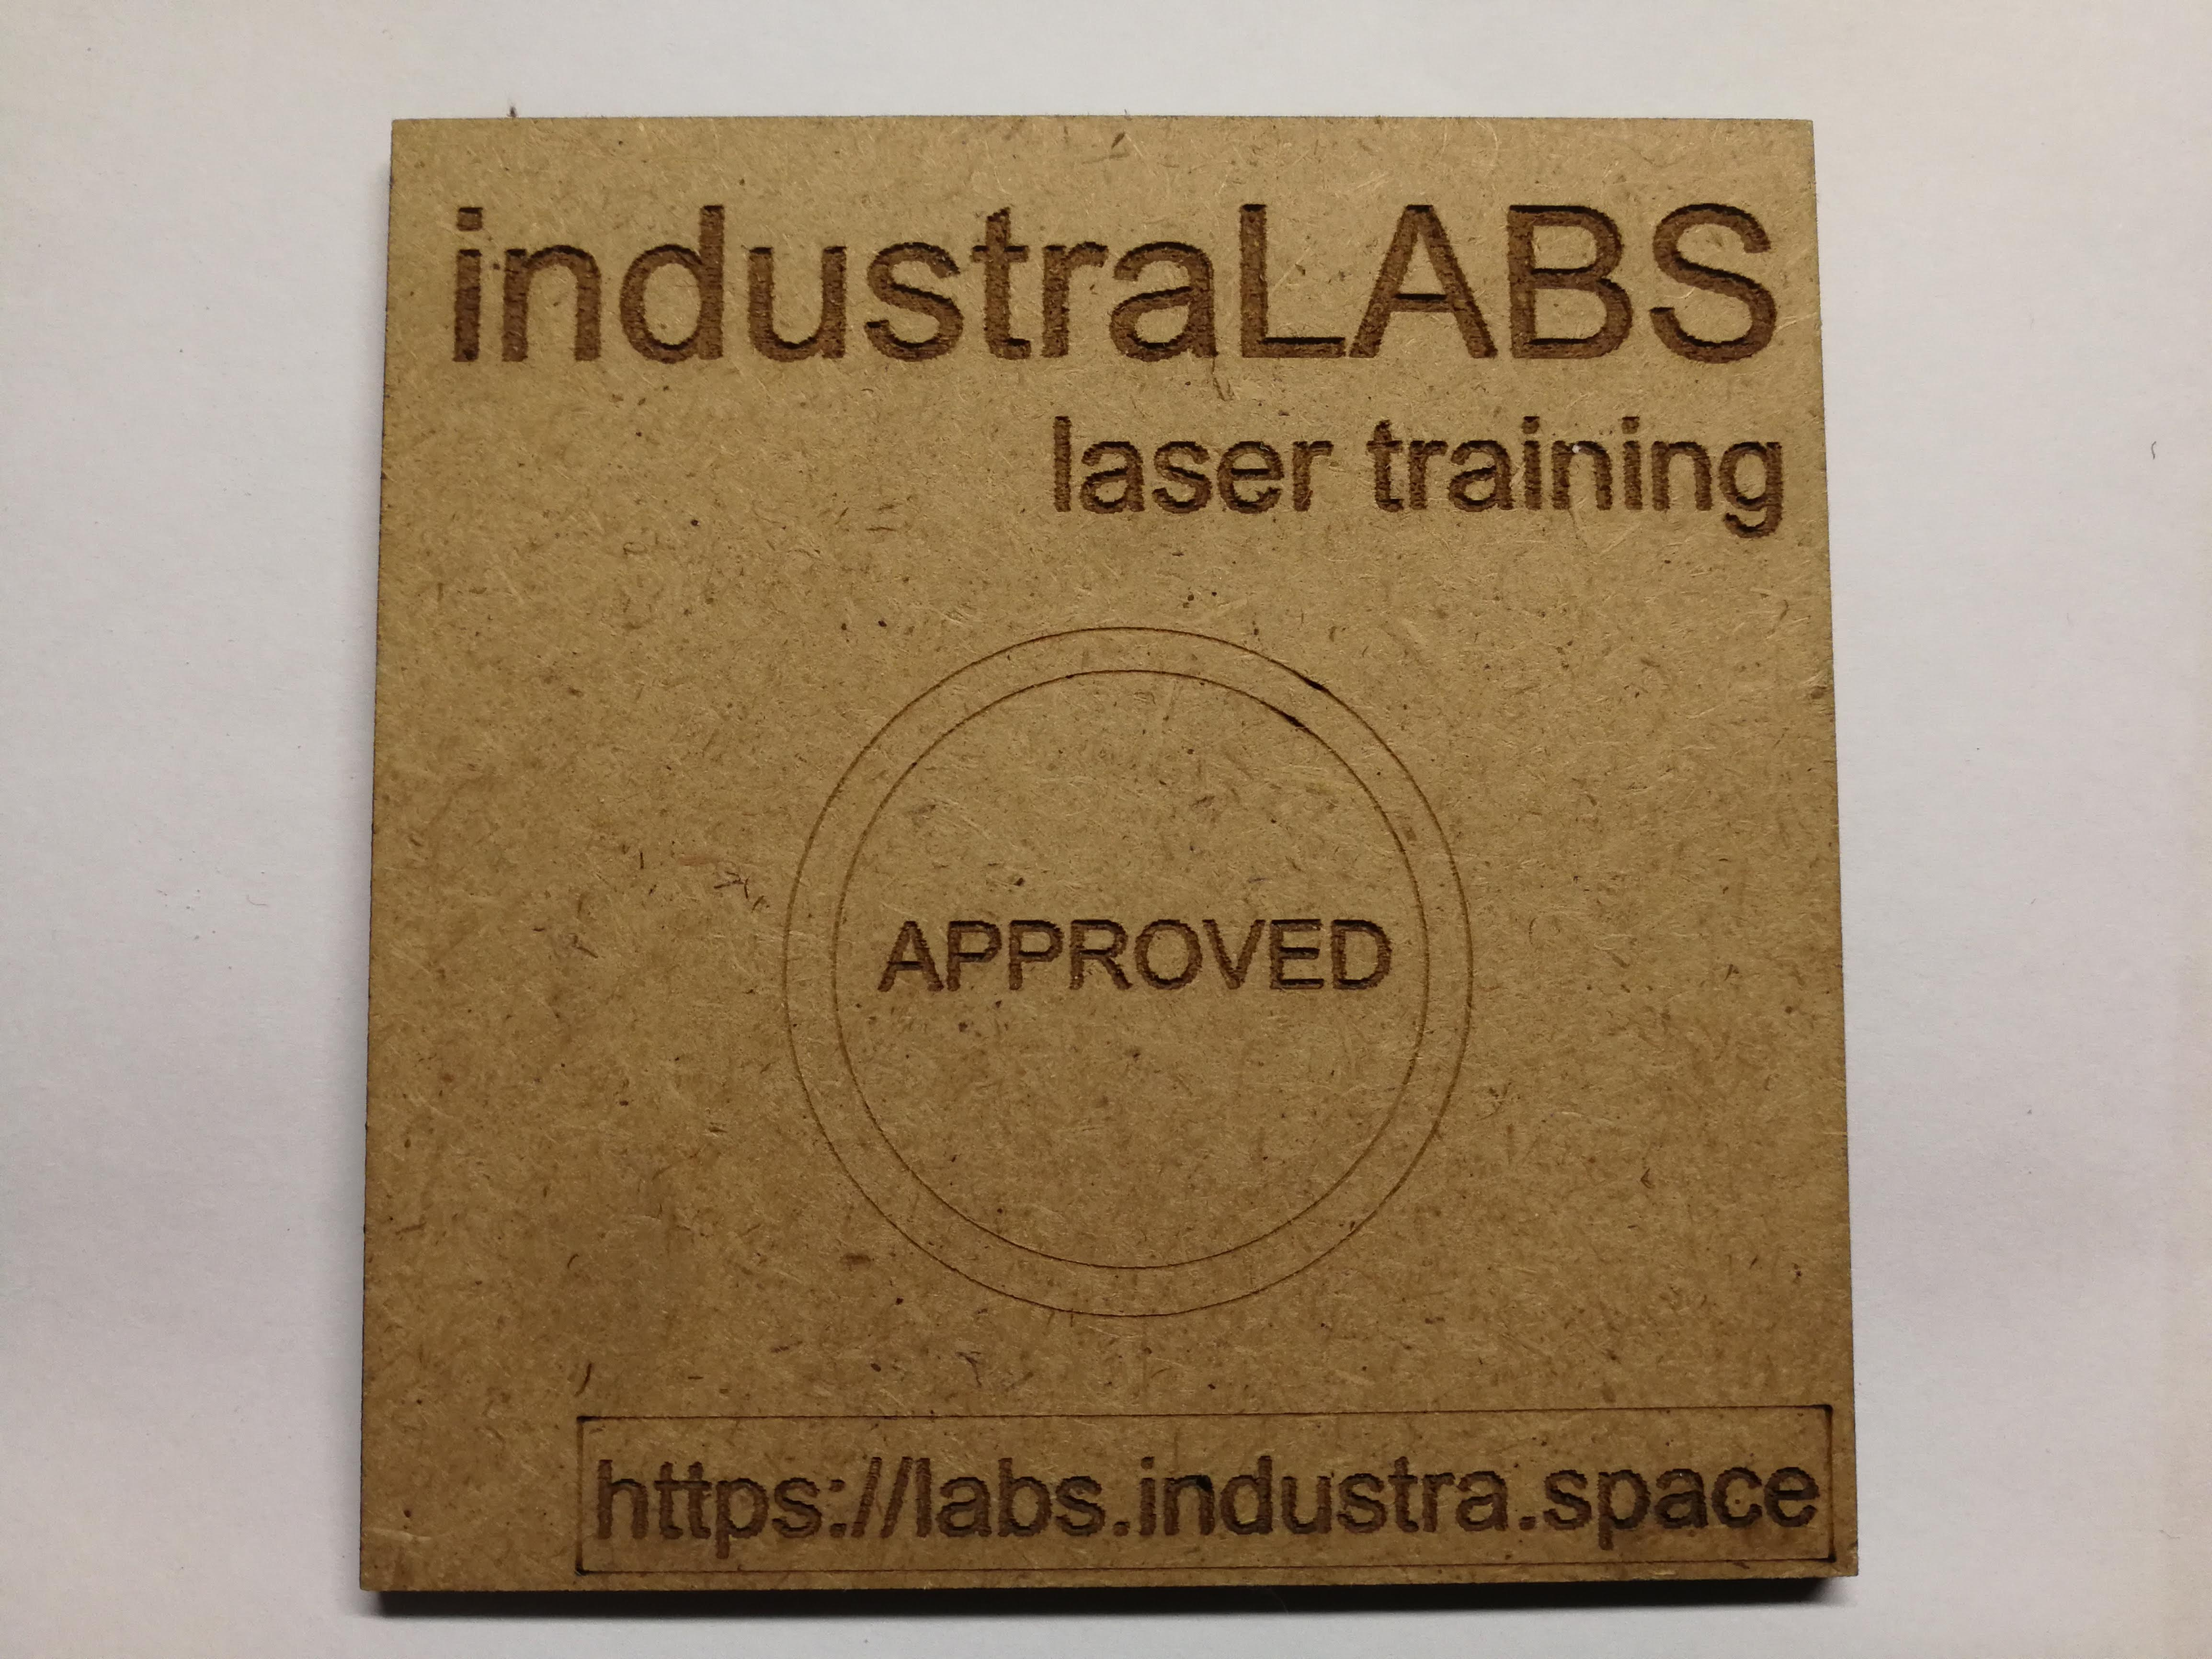
\includegraphics[scale=0.06]{imgs/approved.jpg}
\end{frame}

\section{Teorie}

%---------------------------------------------------------
%Changing visivility of the text
\begin{frame}
\frametitle{Laser}

\begin{block}{ThunderLaser Nova63}
\begin{itemize}
\item řezání (line) a gravírování (fill) nekovů
\item 120W CO$_{2}$ laser
\item vodní chlazení
%\item<2-> Text visible on slide 2
%\item<3> Text visible on slides 3
%\item<4-> Text visible on slide 4
\end{itemize}
\end{block}

\textbf{Komponenty laseru}
\begin{itemize}
	\item vodní chlazení
	\item ofuk (air assist)
	\item odtah spalin
	
\end{itemize}
\end{frame}


%%% workflow chart



%%% workflow chart end



%---------------------------------------------------------
%%% Materials
\begin{frame}
\frametitle{Materiály}


\begin{examples}{Povolené materiály}
	\begin{itemize}
		\item dřevo
		\item HDF, MDF
		\item překližka
		\item plexisklo
		\item katron, papír
		%\item<2-> Text visible on slide 2
		%\item<3> Text visible on slides 3
		%\item<4-> Text visible on slide 4
	\end{itemize}
\end{examples}




\end{frame}

%%% materials - not allowed
\begin{frame}
\frametitle{Materials}

\begin{alertblock}{Zakázané materiály}
	\begin{itemize}
		\item materiály obsahujicí chlor (toxické výpary)
		\item zrcadlo, meď (včetně PCV, odraz laseru zpět do zdroje)
		\item hobbyglass
		\item polystyren
		\item ABS
	\end{itemize}
\end{alertblock}

\end{frame}



\begin{frame}
\frametitle{Ovládací panel laseru}

\centering
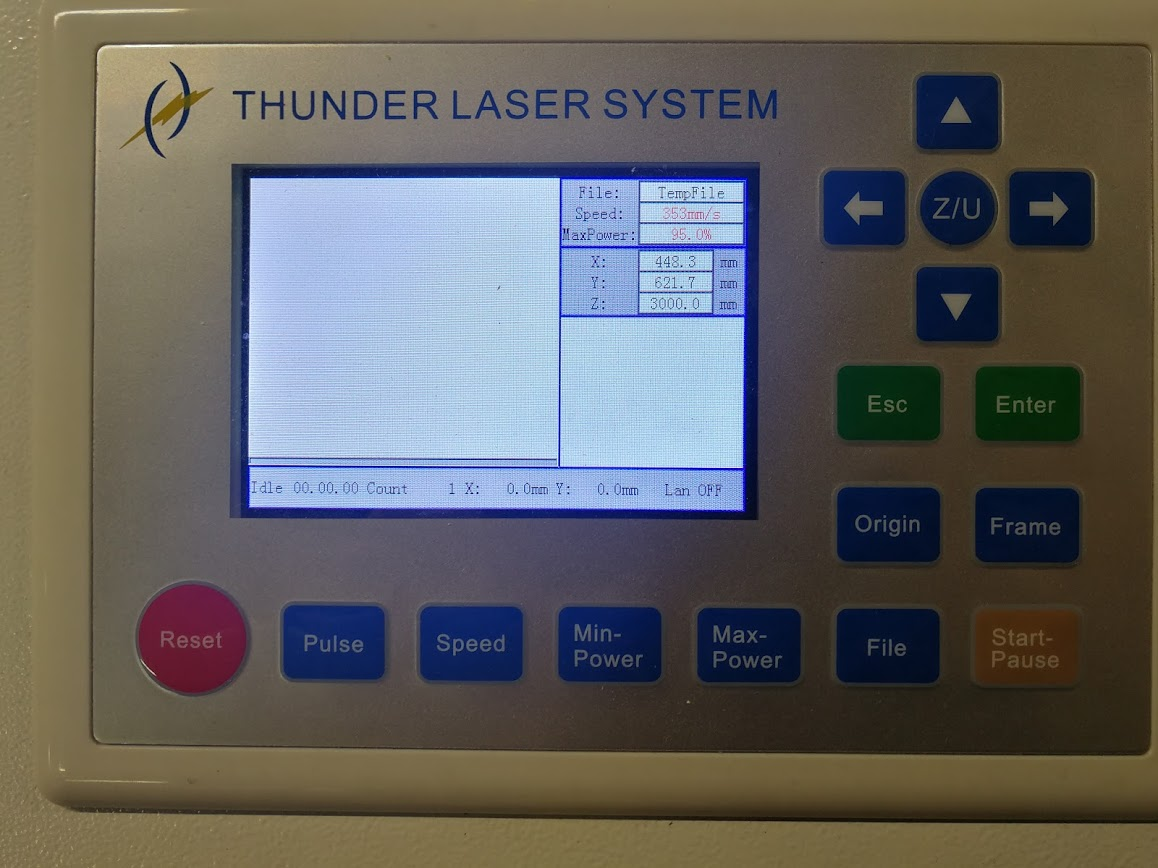
\includegraphics[scale=0.2]{imgs/laser_cp.jpg}

\end{frame}


%% SECURITY
\section{Bezpečnost}
\begin{frame}
\frametitle{Bezpečnost}

\begin{itemize}
	\item nedívejte se na pracující laser bez přestávek
	\item mějte ruce mimo pracovní prostor laseru při pohybu stolu nebo laserové hlavy
	\item nemanipulujte s částmi laseru (vyjma explicitně povolených, jako výměna laserové hlavy)
\end{itemize}

\begin{alertblock}{Použijte červené tlačítko STOP}
	\begin{itemize}
		\item v případě požáru
		\item v případě neočekávaného chování/zvuků
	\end{itemize}
\end{alertblock}

\end{frame}


\begin{frame}
\frametitle{Co je zakázáno}

\begin{itemize}
	\item vypínat ofuk
	\item manipulovat s frekvencí laseru
	\item ovládat laser z vašeho zařízení (na vlastním zařízení je možné připravit Job, ale provést jej je nutné přes naše PC, kvůli správnému nastavení a ovladačům)
\end{itemize}


\end{frame}



\section{Live Demo (Software)}

\begin{frame}
\frametitle{LightBurn}

\begin{itemize}
	\item software pro ovládání laseru
	\item jednoduché operace pro práci s vektorovou grafikou (tvary, text, skupiny, panelizace, bool operace, ...)
	\item import .ai, .dxf, .svg, ... \textit{(vždy je lepší otestovat import na svém zařízení)}
	\item manuální ovládání laseru (nepoužívat)
	\item jednotlivé operace jsou definovány pomocí barev
	\item simulátor
\end{itemize}


\end{frame}

\begin{frame}
\frametitle{Příklad}
\centering

\includegraphics[scale=0.5]{imgs/lb_example.png}

\end{frame}


\begin{frame}
\frametitle{Operace}
\centering
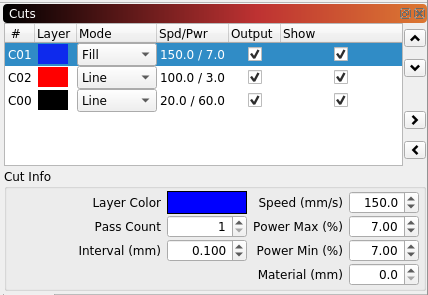
\includegraphics[scale=0.7]{imgs/lb_colors.png}

\end{frame}

\begin{frame}
\frametitle{Simulátor}
\centering
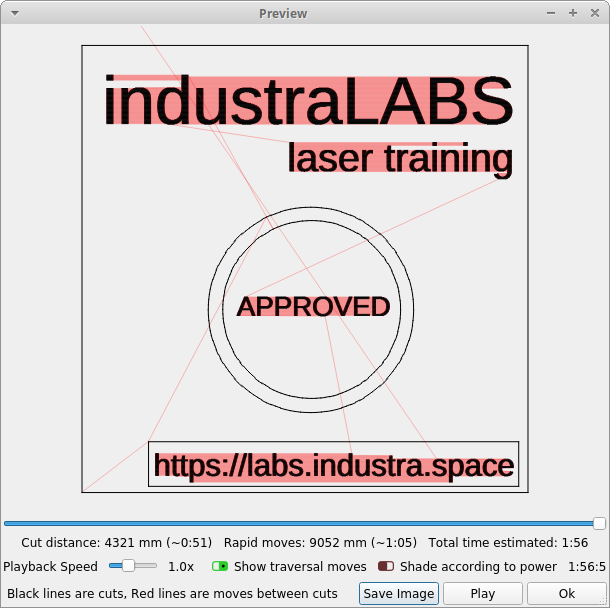
\includegraphics[scale=0.35]{imgs/lb_simulator.png}

\note[item]{vždy dobré použít, předejdete chybám a ztrátě drahého materiálu}
\end{frame}






\section{Live Demo (Hardware)}
\begin{frame}
\frametitle{Live Demo}
\centering
\scalebox{13}{$\leftarrow$}


\end{frame}


\end{document}